\section{Design}
\label{sec:design}

\Syndicate\ is designed with read-heavy but read/write workloads in mind. Motivated by the usage scenarios, this section describes the components of \Syndicate's architecture, shows how these components work together to organize data in a way that is consistent with our observations, and then presents \Syndicate's wide-area data consistency and durability protocols. A common theme throughout the section is to explain how the design makes it easy for \Syndicate\ to leverage independently-operated cloud storage and network caches. The section concludes by discussing several consequences of the design.

\subsection{Components}

\Syndicate\ organizes a user's data into a \textit{Volume}---a collection of data accessible to the user's applications. Objects in the same Volume are replicated to the same set of cloud storage providers, and transferred to readers by the same set of network caches.

Data enters and leaves a Volume via one or more \textit{Gateways}, which are interposed between user application processes, underlying caches and storage, and existing datasets. Each Gateway belongs to exactly one Volume, and operates only on that Volume's data. There are currently three types of Gateways:

\begin{description}

\item[\bf User Gateway (UG):] Interposed between a user application process and the user's Volume. UGs create, delete, read, and write objects on behalf of local processes. UGs host locally-created objects, and (indirectly) serve their data to other UGs through network caches. Our prototype UGs expose a Volume's objects as either a filesystem or a Web object store.

\item[\bf Replica Gateway (RG):] Interposed between a Volume and its cloud storage. UGs replicate object data to cloud storage through Volume RGs. Each Volume has zero or more RGs, and RGs are bound to one or more cloud storage providers. Our prototype RG replicates Volume data to Amazon S3~\cite{S3}.

\item[\bf Acquisition Gateway (AG):] Interposed between a Volume and an existing (external) dataset. Each Volume has zero or more AGs, and each AG is bound to one logical dataset. An AG maps its dataset into the Volume as \Syndicate\ objects for UGs to read. Our prototype imports existing data from either a local file system or from a web server via HTTP.

\end{description}

\noindent The UG configured with a given Volume defines how users interact with the Volume, for example, as a global file system or as a web-based storage service. The next section describes an implementation of both possibilities. This section describes \Syndicate\ in terms of reading and writing abstract data objects.

Note that because the various gateways exchange data indirectly via network caches, it is natural to use HTTP as the underlying data-transfer protocol, implying that \Syndicate\ is effectively an HTTP-based application. The important consequence is that cached objects are named by URLs, with \Syndicate\ responsible for crafting URLs (object names) so as to manipulate caches to meet data consistency requirements, as described later in this section.

\begin{figure}[h!]
\centering
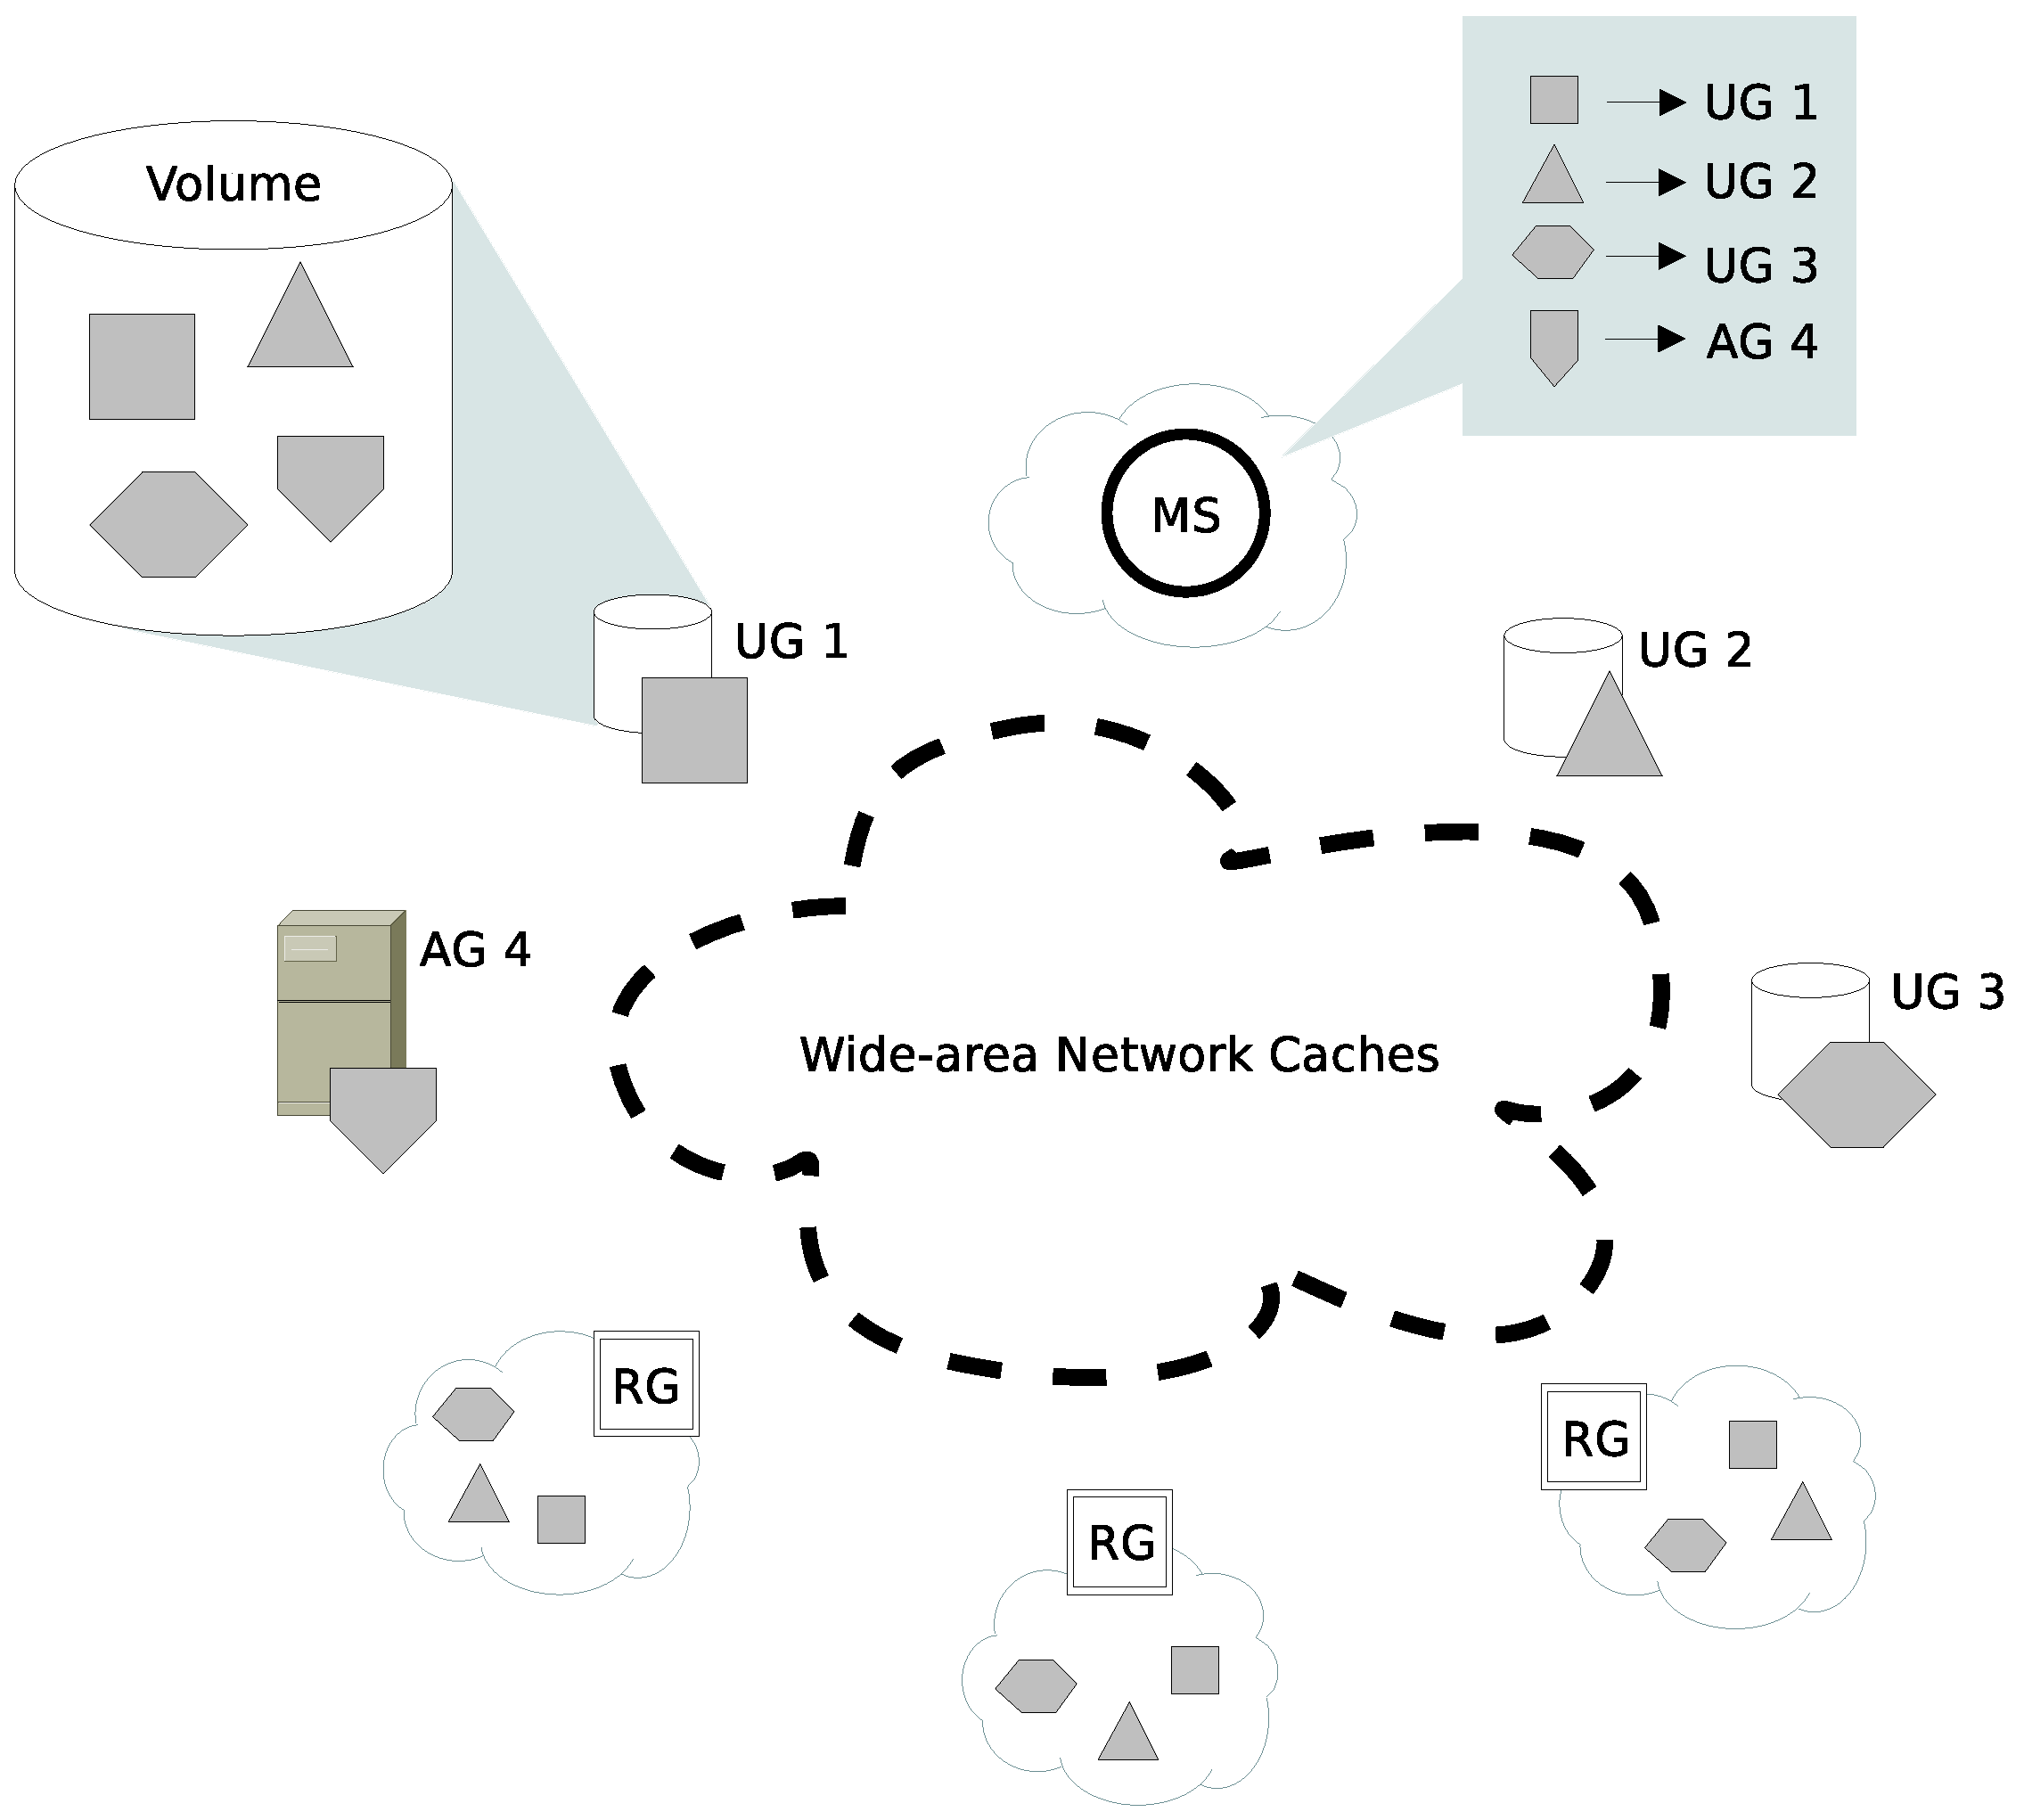
\includegraphics[width=0.5\textwidth]{figures/components}
\caption{\it Each UG presents a view of all objects in a Volume.  RGs upload and download replicated objects from cloud storage.  AGs present existing datasets as objects in the Volume.  Gateways synchronize with the MS to discover the Volume configuration and objects, and read data from one another through wide-area network caches.}
\label{fig:architecture}
\end{figure}

The final \Syndicate\ component is a {\it Metadata Service (MS)}, which the Gateways use to coordinate access to the Volume. The MS is a scalable cloud-hosted service that enforces the binding between the Gateways and their Volume. It stores and serves metadata for each object in each Volume, and ensures that an object name identifies at most one object in a Volume. In doing so, it provides the other \Syndicate\ components an authoritative model of the system.

\subsection{Data Organization}

User-created objects are maintained by a UG that serves as its \textit{acting owner}. In the absence of failures, the UG that created an object serves as it's acting owner. This lets users place objects across the wide-area in a domain-specific manner.

The acting owner UG hosts the object's data locally and serves (sources) it to the Volume's other gateways, indirectly through any available network caches. This lets a scalable number of remote reader UGs access the data while providing good read and write performance to local processes.

A UG reads non-local object data by requesting it, first from the acting owner UG, and then from the Volume's RGs if the acting owner cannot be reached. The UG constructs the request for a non-local object in such a way that the caching substrate is able intercept and serve the content. The caches in this substrate, in turn, request the data from the corresponding source upon a cache miss.

A UG writes to a non-local object by committing the written data to its local storage, and then synchronously informing the object's acting owner UG that a write has taken place. This message is small relative to the size of the write, and ensures that an acting owner UG sees all writes on its objects in some sequential order. This additionally lets the UG handle writes that expand the size of the object, as well as handle append-only write semantics.

On receipt of a remote write message, the acting owner UG directs subsequent requests for the object's modified data to the writer UG. On local read, it fetches the modified data from the writer UG---indirectly through the caching substrate---and resumes hosting it. We say that the acting owner UG has ``re-integrated'' the modifications in this case. It then asynchronously informs the writer UG that it no longer has to store the modifications.

This data organization scheme works well when non-local data is likely hosted in a nearby cache (i.e. when there are many reads on the object). This allows UGs to store written object data locally (and thus quickly) regardless of whether or not they are the object's acting owner, because the cost of fetching the modified data is amortized across many subsequent cache hits.

\subsection{Metadata Organization}

UGs discover objects through the MS. When an acting owner UG creates, deletes, or updates an object (i.e. when handling a write on behalf of an application process), it sends its object's new metadata to the MS. Reader UGs later contact the MS to discover objects and detect when they have changed.

While the MS is a logically central service, it is designed to scale with the number of UGs and objects. It runs in a wide-area environment across a cloud platform's datacenters and computing nodes. In order to maximize a user's flexibility in determining the structure of their data while preserving this scalability, it organizes data into a flat namespace via a key/value store.  To ensure that no two objects may share the same name, the MS specifically leverages an indexed key/value store (i.e. a NoSQL store) that offers support for transactions across two related keys, and provides at least one secondary index. This lets the MS take advantage of the storage scalability, availability, and partition tolerance offered by a good NoSQL store implementation~\cite{bigtable,hyperdex}, provided the MS organizes its data appropriately.

There are two design challenges of the MS. First, the MS must organize object metadata records such that it can host a scalable number of metadata records while allowing a scalable number of UGs to read and write them simultaneously. Second, the MS must ensure that an object name refers to at most one object.

We designed the MS to store a small, fixed amount of data per metadata record. This greatly simplifies the task of distributing record data throughout the store and makes it easier to cache records. \Syndicate\ does this by dividing an object's metadata between the MS its acting owner UG. The MS stores a set of common, fixed-length attributes in each object's metadata record. This includes a user-chosen identifier, a \Syndicate-chosen key, a key to another metadata record, and an identifier of the object's acting owner UG. The acting owner UG stores the remaining metadata for its object---in effect, a \textit{manifest} of the object's content---which can grow linearly with the size of the object, as described in the next section.

To allow the MS to read and write a scalable number of records at once, it logically organizes a Volume's metadata records into a directed graph with object records and ``directory'' records as vertices. There is an edge $a \rightarrow b$ if record $a$ is the parent of $b$. Only a directory can be a parent. Object records have no incoming edges, but every directory record has zero or more incoming edges and exactly one outgoing edge. There is a single ``root'' directory whose outgoing edge refers to itself. Each record stores the key to its parent.

A record is named by its Volume's identifier and the sequence of record identifiers along the reversed path from the root to the record. This makes it easy to compute a parent record's name from the record's name. A record's key is generated from its name.

Using this organization, creating a record such that its name only identifies this record is a matter of ensuring that the parent directory record exists, and that this record's key has not been mapped to a value in the store. As an atomic operation (a transaction across two keys), the MS performs these checks, and if successful, maps the record key to the record data, updates the last-modified time of the parent, and increments a parent's count of the number of records that rely on it as a parent.

The MS updates and deletes a record using a similar transaction to creation.  A directory record will not be deleted if it is the parent of at least one record (as indicated by its counter). Reads on a record may be concurrent with one another and with ongoing transactions, but they return record data as it was before a concurrent transaction began.

The effect of this organization is that there can be as many concurrent metadata writes in a Volume as there are disjoint record/parent pairs. There can be as many concurrent reads as the store supports. Directory records are created by users (via their UGs), which allows them to control object naming, data organization, metadata organization, and write concurrency. Through careful directory organization, there can be as many concurrent metadata writes as there are objects. Furthermore, ths organization can be leveraged for data consistency, as discussed in the next section.

To read an object, a UG only needs to know its name and Volume to generate its key. To discover objects, a UG only needs to know the root's name and Volume. It can then perform a breadth-first search of the MS's records by iteratively finding all records with the current directory's key listed as the parent. To facilitate this, the MS leverages the underlying store to keep a secondary index on the parent key field, and leverages a distributed coherent cache in the cloud (such as memcache~\cite{memcache}) to store and quickly return frequently-requested queries.

\subsection{Consistency}

The UG data organization scheme naturally lets the acting owner UG resolve write conflicts on an object in an implementation-specific manner (e.g. our prototypes use a last-write-wins~\cite{last-write-wins} policy, but others are possible). The challenge is how to design the UG to detect when data in network caches is stale, and take steps to pull fresh data into the caches.

\Syndicate's data consistency protocol leverages the fact that network caches identify data by an object-specific name (i.e. a URL). Suppose the acting owner UG were to create a globally-unique URL for an object before a write completes, and that a remote reader UG could discover the URL associated with the last write before reading data from a network cache. Then, the reader UG will receive data consistent with all write operations up to the write operation that caused the given URL to be generated.

This approach works well for small objects, but will cause cache thrashing with large objects. This is because small modifications will cause readers to pull multiple versions of the large object into the caches, potentially evicting many smaller objects. To avoid this problem, the acting owner UGs distributes globally-unique URLs for only modified regions of object data. Then, reader UGs collect these URLs to reconstruct object data from previous modifications, allowing them to pull modified bytes into network caches and hit unmodified bytes still in the cache.

There are three critical considerations that make this difficult in the wide-area:
\begin{itemize}
\item The metadata required to track modifications cannot grow so large as to make it difficult for acting owners to generate new URLs for readers.
\item There must be a fast way to propagate these URLs to a scalable number of readers, despite the fact that an acting owner UG might run on an under-provisioned edge network.
\item The metadata must be available for reads and writes when the acting owner UG goes offline.
\end{itemize}

The approach taken by \Syndicate\ is to break each object's data into a sequence of fixed-sized blocks. Each block has a randomly-generated version unique to each write operation that affected it, and the object has a monotonically-increasing version unique to its generation. Acting owner UGs host and track this metadata by organizing it into a manifest.

An object's \textit{manifest} is a compact range data structure that stores enough information for any UG to generate a globally-unique URL for any block in the object as of the last write. To do this, the manifest stores the object's name, version, block number, block version, and identifier of the Gateway that hosts each block.\footnote{A UG resolves the identifier to the Gateway's URL. UGs periodically download and cache a mapping between Gateway identifiers and their URLs from the MS, in order to help keep manifests compact.} A block URL contains all of this information, making it globally unique to each write (with high probability).

\begin{figure}[h!]
\centering
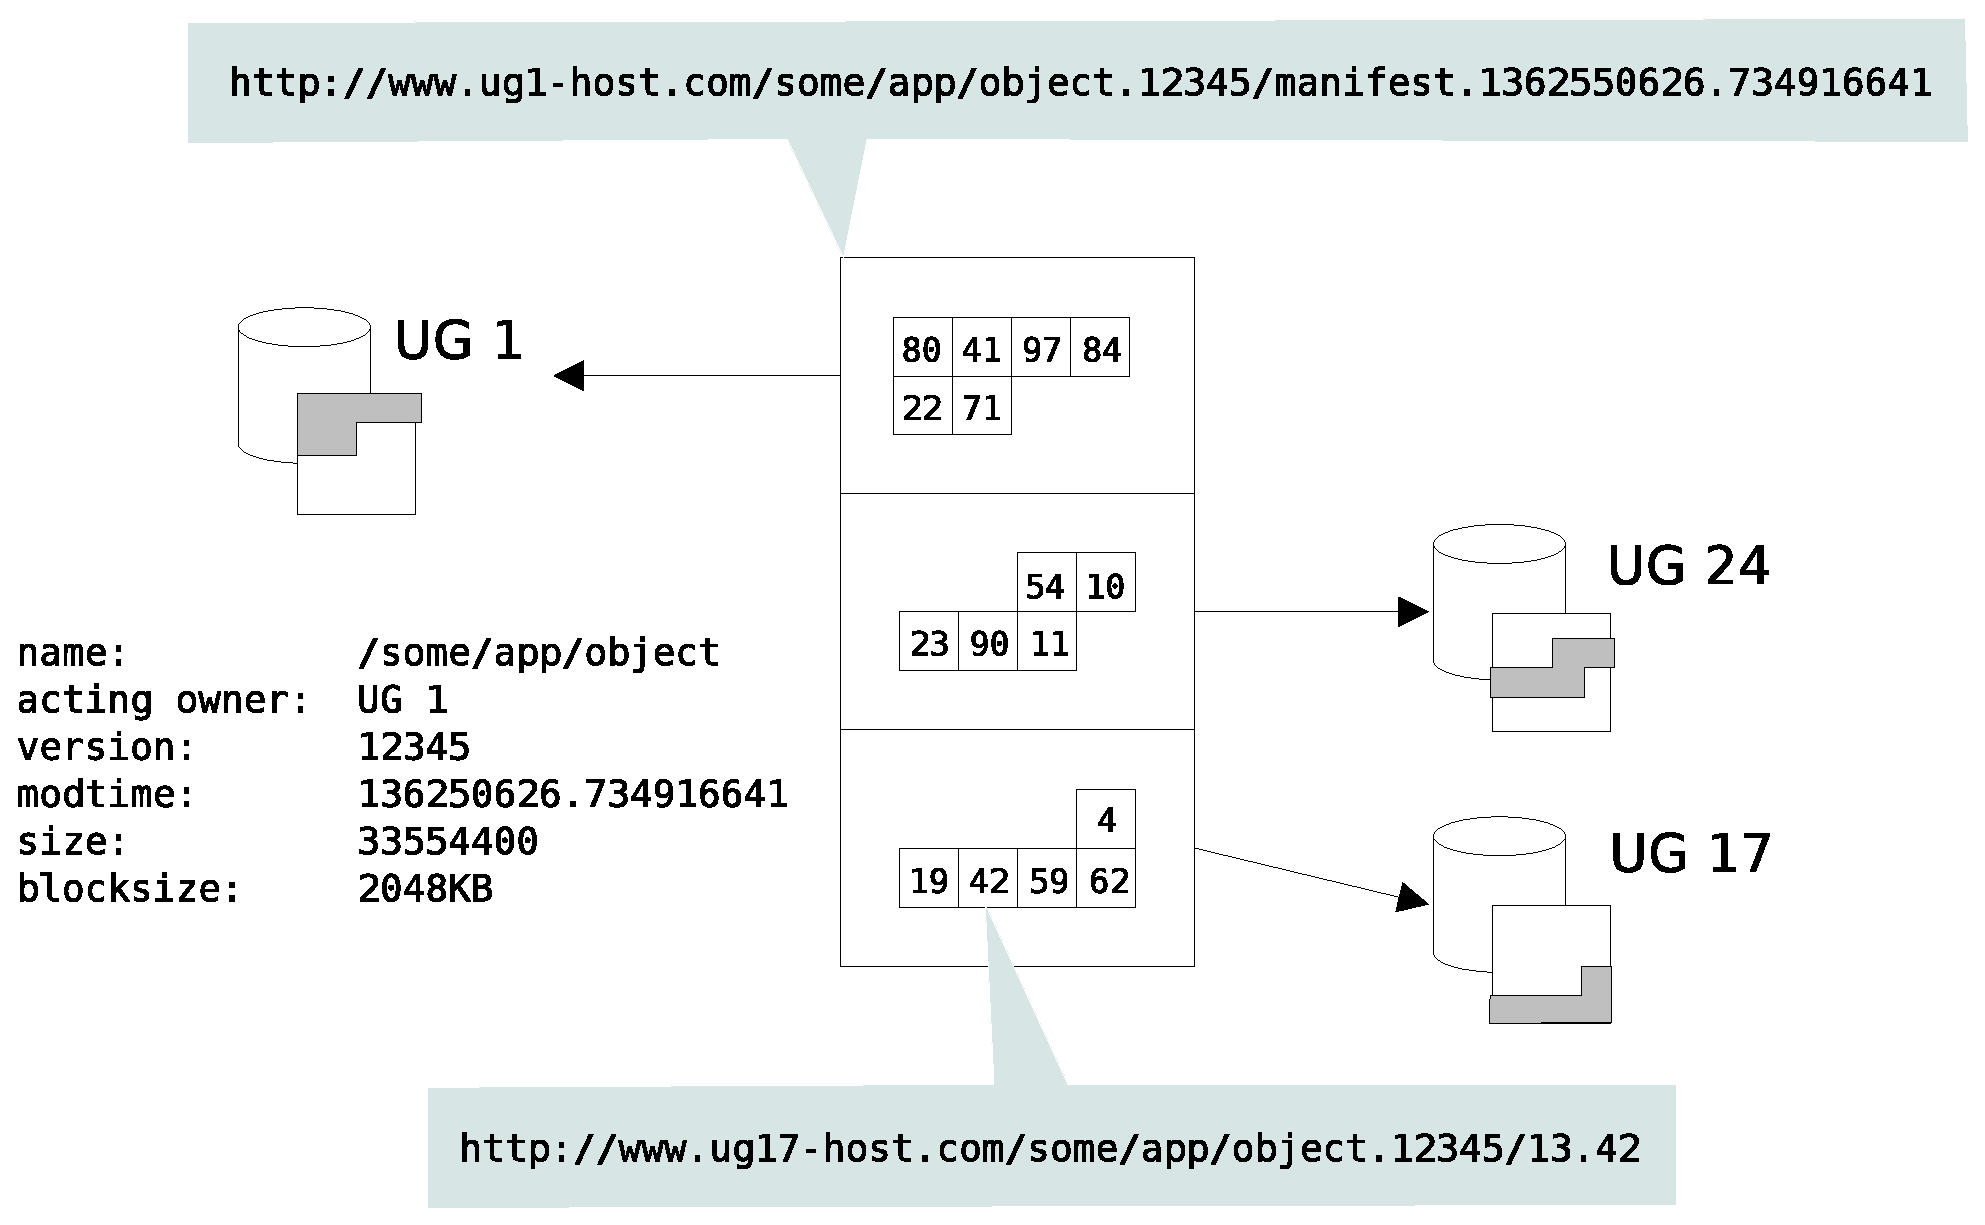
\includegraphics[width=0.5\textwidth]{figures/manifest}
\caption{\it Logical representation of a manifest, including manifest and block URL generation.  UG 1 is the acting owner of the object, and UGs 24 and 17 have written new blocks.  For brevity, block versions in this figure are between 0 and 99, but in practice the range would be sufficiently large to avoid duplicate version numbers across the object's lifetime.}
\label{fig:architecture}
\end{figure}

The acting owner UG uses the manifest to locate the object's blocks to service local reads, as well as to redirect remote reads to Gateways that host remote blocks. When a UG writes data (either locally or remotely), it atomically generates new block versions and updates its copy of the manifest. Remote writers send their new block versions to the acting owner UG as part of the write operation, so the acting owner UG can direct subsequent reads appropriately.

Each range in the manifest represents the versions of a contiguous region of blocks that are hosted on a single Gateway. This means that when serialized into a message, a manifest's size is a small constant multiple of the number of blocks in an object, plus the number of different Gateways hosting data (which itself is at most the number of blocks in the object). We expect users to pick a relatively large block size relative to the number of blocks (no smaller than on the order of tens of kilobytes) to maximize network protocol goodput and cache goodput.

To ensure reader UGs discover the URLs to fresh object data, we must ensure that they have fresh copies of the object's manifest. When an active owner UG modifies an object's manifest in any way, it informs the MS that it has done so by uploading the nanosecond-resolution time of modification. The MS keeps this timestamp with its portion of the object's metadata record.

Later, interested readers request its metadata from the MS. They use the metadata to generate a URL for the object's manifest, and request the manifest from the acting owner UG, indirectly through the caching substrate. The timestamp resolution and object version both ensure with high probability that the manifest URL will be globally unique, meaning that the manifest data received from the cache will be consistent with the write at the modification time. Once they have the fresh manifest, readers generate globally-unique block URLs that correspond to the written data and request them from the caches.

With concurrent reads and writes on the same object, there is a chance that a generated URL will refer to stale data by the time the request is sent. This happens if a write on the requested object data starts and completes between when the reader obtains the URL to the data and when the reader begins requesting the data. The result is that the read could return a copy of data as it was before the write (i.e. stale data). Whether or not this happens depends on whether or not the requested data was cached.

If the requested data is not cached, the request is sent to the acting owner UG via a cache miss. However, because the URL contains the object's version, and either the manifest timestamp or the block version, the acting owner UG can tell that it refers to stale data. In this case, it simply redirects the reader to a fresh URL for the data, and the reader tries again.

If the requested data was cached after all, then the reader receives stale data. However, because the acting owner UG serialized all writes on the object, the stale data will be consistent with all prior writes except for the writes that were concurrent with the read (i.e. the writes occurred after the reader obtained the URL but before it began requesting data).

If the user cannot avoid concurrent reads and writes on an object, \Syndicate\ offers the user two ways to control staleness. First, it lets users place a time bound on how long a reader's URLs will be valid (i.e. it provides per-object delta consistency~\cite{delta-consistency}). Second, it lets users implement mutual exclusion protocols by leveraging the fact that the MS ensures that an object name refers to at most one object.

To provide delta consistency, the MS stores for each object a user-determined delta ($\Delta_{read}$) in milliseconds. The reader UG uses $\Delta_{read}$ to determine for how long after download a local copy of an object's metadata (including its manifest) is considered fresh. Metadata older than this will be synchronously re-downloaded from the MS and acting owner UG when next used.

With this scheme, reader UG $A$ will receive fresh data from an object's acting owner UG $B$ by waiting $\Delta_{read} + RTT_{MS} + RTT_{AB} + \varepsilon$ milliseconds after a write (where $\varepsilon$ is RTT measurement error). Users can trade read performance for less stale data by choosing smaller $\Delta_{read}$ values. The performance penalty comes from the more frequent RTTs to the MS and the acting owner.

\subsection{Durability and Fault Tolerance}

By default, object data written by any UG is synchronously replicated to its Volume's RGs before the write completes. An acting owner UG synchronously replicates an object's manifest to the RGs whenever it changes, but only after all modified blocks have been replicated. The UG uploads a manifest's modification time to the MS only after the manifest has been replicated.

The RG is effectively a cloud storage ``driver'' for \Syndicate. It receives blobs of data from authorized UGs, and uploads the data to cloud storage under a UG-given name (i.e. the path component of the block or manifest URL). On a subsequent request for data, it fetches and serves the blob from cloud storage named by the URL path of the request.  The RG authorizes UGs by coordinating with the MS (see Section~\ref{sec:composition}).

If an acting owner UG goes offline, reader UGs can continue to read its objects by requesting the latest manifests and blocks from Volume RGs. By ensuring that a new manifest can only be discovered after the manifest and blocks have been replicated, an acting owner UG ensures that reader UG can rely on the RGs to serve data consistent with writes.

If a writer UG attempts to write to a remotely-hosted object, and it discovers that the acting owner UG is offline, it attempts to become the new acting owner. First, it downloads the latest manifest from the RGs, and updates it to list an RG as the Gateway that hosts the dead owner's local blocks. Second, it asks the MS to update the object's metadata record to refer to it as the new acting owner.

To ensure object ownership stabilizes in the face of many writes, the writer UG sends the identifier of what it believes to be the current acting owner UG along with the request. If the identifier matches the acting owner UG in the MS's object record, the MS makes the writer UG the new acting owner. If it does not match, the MS sends the writer UG the identifier of the new acting owner UG, and the writer UG sends its write message to the new acting owner instead.

If the writer UG succeeds at becoming the new acting owner, it writes its data locally, updates the manifest, replicates the new manifest and modified blocks, and updates the object's timestamp on the MS. It serves as the acting owner until either it fails (in which case the above protocol is repeated to find a new acting owner), or the original owner comes back online.

If the original owner comes back online, it first determines the current acting owners of its objects using the MS. It then requests that each acting owner relinquish the object by sending it the current manifest and directing subsequent reads and writes to it. The owner then updates the object metadata on the MS to refer to it as the new acting owner.

\subsection{Service Composition}

As part of a Volume's configuration state, the MS maintains a list of which Gateway instances interact with Volume data. Each Gateway has a set of authentication credentials that it presents to the MS on each metadata operation, so the MS can prevent unauthorized metadata access. The credentials are randomly generated when a Gateway is added to the Volume, and are revoked when a Gateway leaves a Volume. The user supplies the Gateway with its credentials when it starts up.

\subsubsection{Reconfiguration}

Each version of the Volume's configuration state has a unique nonce, generated from the configuration's cryptographic hash and the current time on the MS. A Gateway includes this nonce along with each message it sends, and it rejects messages from other Gateways with an incorrect nonce. If a message is rejected due to an invalid nonce, a Gateway refreshes the nonce from the MS and downloads new relevant configuration state. If a Gateway is removed from the Volume, the refresh will fail and the Gateway will die.

To prevent the nonce from being intercepted by eavesdroppers, each Gateway encrypts messages sent to other Gateways. A Gateway prevents nonces from being seen by network caches and cloud storage.

\subsubsection{Composition}
\label{sec:composition}

The reconfiguration protocol allows the user to dynamically add and remove Gateways and infrastructure in a Volume, and have other Gateways discover and use them. 

To add a network cache to a Volume, a user uploads its HTTP proxy URL (and optionally HTTP authentication credentials) to the MS as part of the Volume's configuration state. Most network caches are meant for use with the Web and implement an HTTP proxy interface~\cite{HTTP-RFC}, but nonstandard caches can be made available to the Volume by interposing a specially-crafted HTTP proxy to perform protocol translation. UGs discover the latest set of network cache URLs when they refresh their nonces. Similarly, an entire distributed collection of network caches---that is, a CDN---can be integrated into a Volume by configuring the URL-prefix that causes requests to be redirected to the CDN (e.g., \texttt{www.coblitz.org}), where the CDN is responsible for redirecting each request to the specific cache that can best serve that request.

To add a cloud storage provider to a Volume, a user first instantiates a corresponding RG and adds the URL for the RG to the Volume's configuration state. Then, UGs discover the latest set of RGs and proceed to use them when they refresh their nonces.

A RG refreshes its nonce when it receives a replication request from a UG with a nonce it has not seen before. If the current nonce does not match the UG's nonce, it will deny the replication request.

To map existing datasets into a Volume as read-only objects, a user first instantiates the appropriate AG. On start-up, the AG creates object records on the MS that will refer to different portions of its dataset. The AG generates manifests for its objects to serve to UGs, and translates block URL requests into the appropriate data.

The precise organization of an AG's objects is specific to the AG implementation and dataset. The MS differentiates between AG-created records and UG-created records, so that when an AG is removed from the Volume, its records are removed as well.

\subsection{Discussion}

There are several consequences to \Syndicate's design. First, read and write performance in \Syndicate\ is largely predictable from underlying storage and caches. The only differences between using \Syndicate\ and using the underlying mechanisms directly are the effects of \Syndicate's consistency and durability protocols, which an application not using \Syndicate\ would have to address on its own.

Another consequence is that a user can enforce cache utilization policy by interposing a specially-crafted HTTP proxy between UGs and the underlying caches. For example, an HTTP proxy could rate-limit a UG, redirect requests to multiple different network caches based on measured cache performance, send requests directly to a UG for uncacheable data, and so on. This benefit is a direct consequence of using the RESTful HTTP protocol.

Similarly, a user can leverage a specially-crafted RG to enforce utilization policy on \Syndicate's cloud storage providers. For example, an RG can store certain data only to a trusted cloud, if the object is named to indicate that it contains sensitive information. As another example, a specially-crafted AG can impose read access control through permission bits in its objects' MS records. Because HTTP proxies, RGs and AGs can be added and removed dynamically, the user can interpose usage policy at runtime.

Because of its interface's simplicity, a RG can transparently route requests to other RGs, and aggregate RG responses. This presents an opportunity for implementing many different replication schemes by composing RG processes, while presenting a logically-singular RG to a Volume. For example, a horizontally-scalable RG implementation could use DNS redirection to load-balance replication requests across many subordinate RGs, and dynamically instantiate additional RG processes as replication demand increases.

Finally, because \Syndicate\ leverages an underlying indexed key/value store for hosting its metadata, users are not limited to organizing their data hierarchically.  Although we implemented a prototype UG that organizes data into a filesystem, alternative implementations can organize data in a much more general manner.  The directory record in \Syndicate\ only exists to provide a serialization point for related objects, instead of imposing a hierarchy.

